\documentclass[a4paper,10pt]{article}
\usepackage[utf8]{inputenc}
\usepackage{amsmath}
\usepackage{amssymb}
\usepackage{graphicx}
%für quellcode
\usepackage{listings} 

\newcommand{\image}[3]{\begin{figure}[h]
                            \includegraphics[#1]{#3}
                            \caption{#2}
                       \end{figure}
                       }

\lstset{
    language = octave
}
%begin{lstlisting}

\begin{document}
%########################################
%		Titel
%########################################
\begin{center}
    \section*{Mustererkennung Übungszettel}
     \today
\end{center}
$ $
\newline
\begin{tabular}{r|l l}
    Name & Alexander Hinze-Hüttl & Kevin Pandura\\
    Matrikelnummer & 4578322 & 4562742\\
\end{tabular}
\newline
$ $
\newline
\newline
%########################################
%		Ende
%########################################

\section{Aufgabe 1}
	Berechnen die Wahrscheinlichkeit, dass bei $x$ Metern ein Tor erzielt
	wird mittels $\beta$:
	\begin{lstlisting}
function w = p(x,b)
   extendedX = [x;1];
   w = exp(transpose(b)*extendedX)/(1+exp(transpose(b)*extendedX));
endfunction
	\end{lstlisting}
	Berechnen Gradientenabstieg mittels:
	\begin{lstlisting}
newbeta = beta + a * lBeta(beta,data);
	\end{lstlisting}
	Wobei $\nabla l(\beta)$ wie folgt implementiert wurde:
	\begin{lstlisting}
function b = lBeta(beta,data)
  b = 0;
  [h,w] = size(data);
  for i = 1:h
    x = data(i,1);
    y = data(i,2);
    b += [x;1]*(y - p(x,beta));
  endfor
endfunction
	\end{lstlisting}
	Leiter dauert das Iterieren bis $100.000$ unheimlich lange und da
	wir keinen leistungsstarken Rechner besitzen, iterieren wir $k = 1:1000$:
	\\
	\texttt{
		k = 250, beta = (0.029591,0.002054) error = 351.866106 color = red\\
		k = 500, beta = (0.029614,0.003335) error = 351.641306 color = green\\
		k = 750, beta = (0.029580,0.004614) error = 351.614392 color = blue\\
		k = 1000, beta = (0.029546,0.005893) error = 351.587984 volor = black
	}
	\\
	Für $k=1:100.000$ reichen wir gerne Ergebnisse nach, wenn wir mehr Zeit für die Rechnung haben.
	\\
	Leider wächst unsere Kurve:\\
	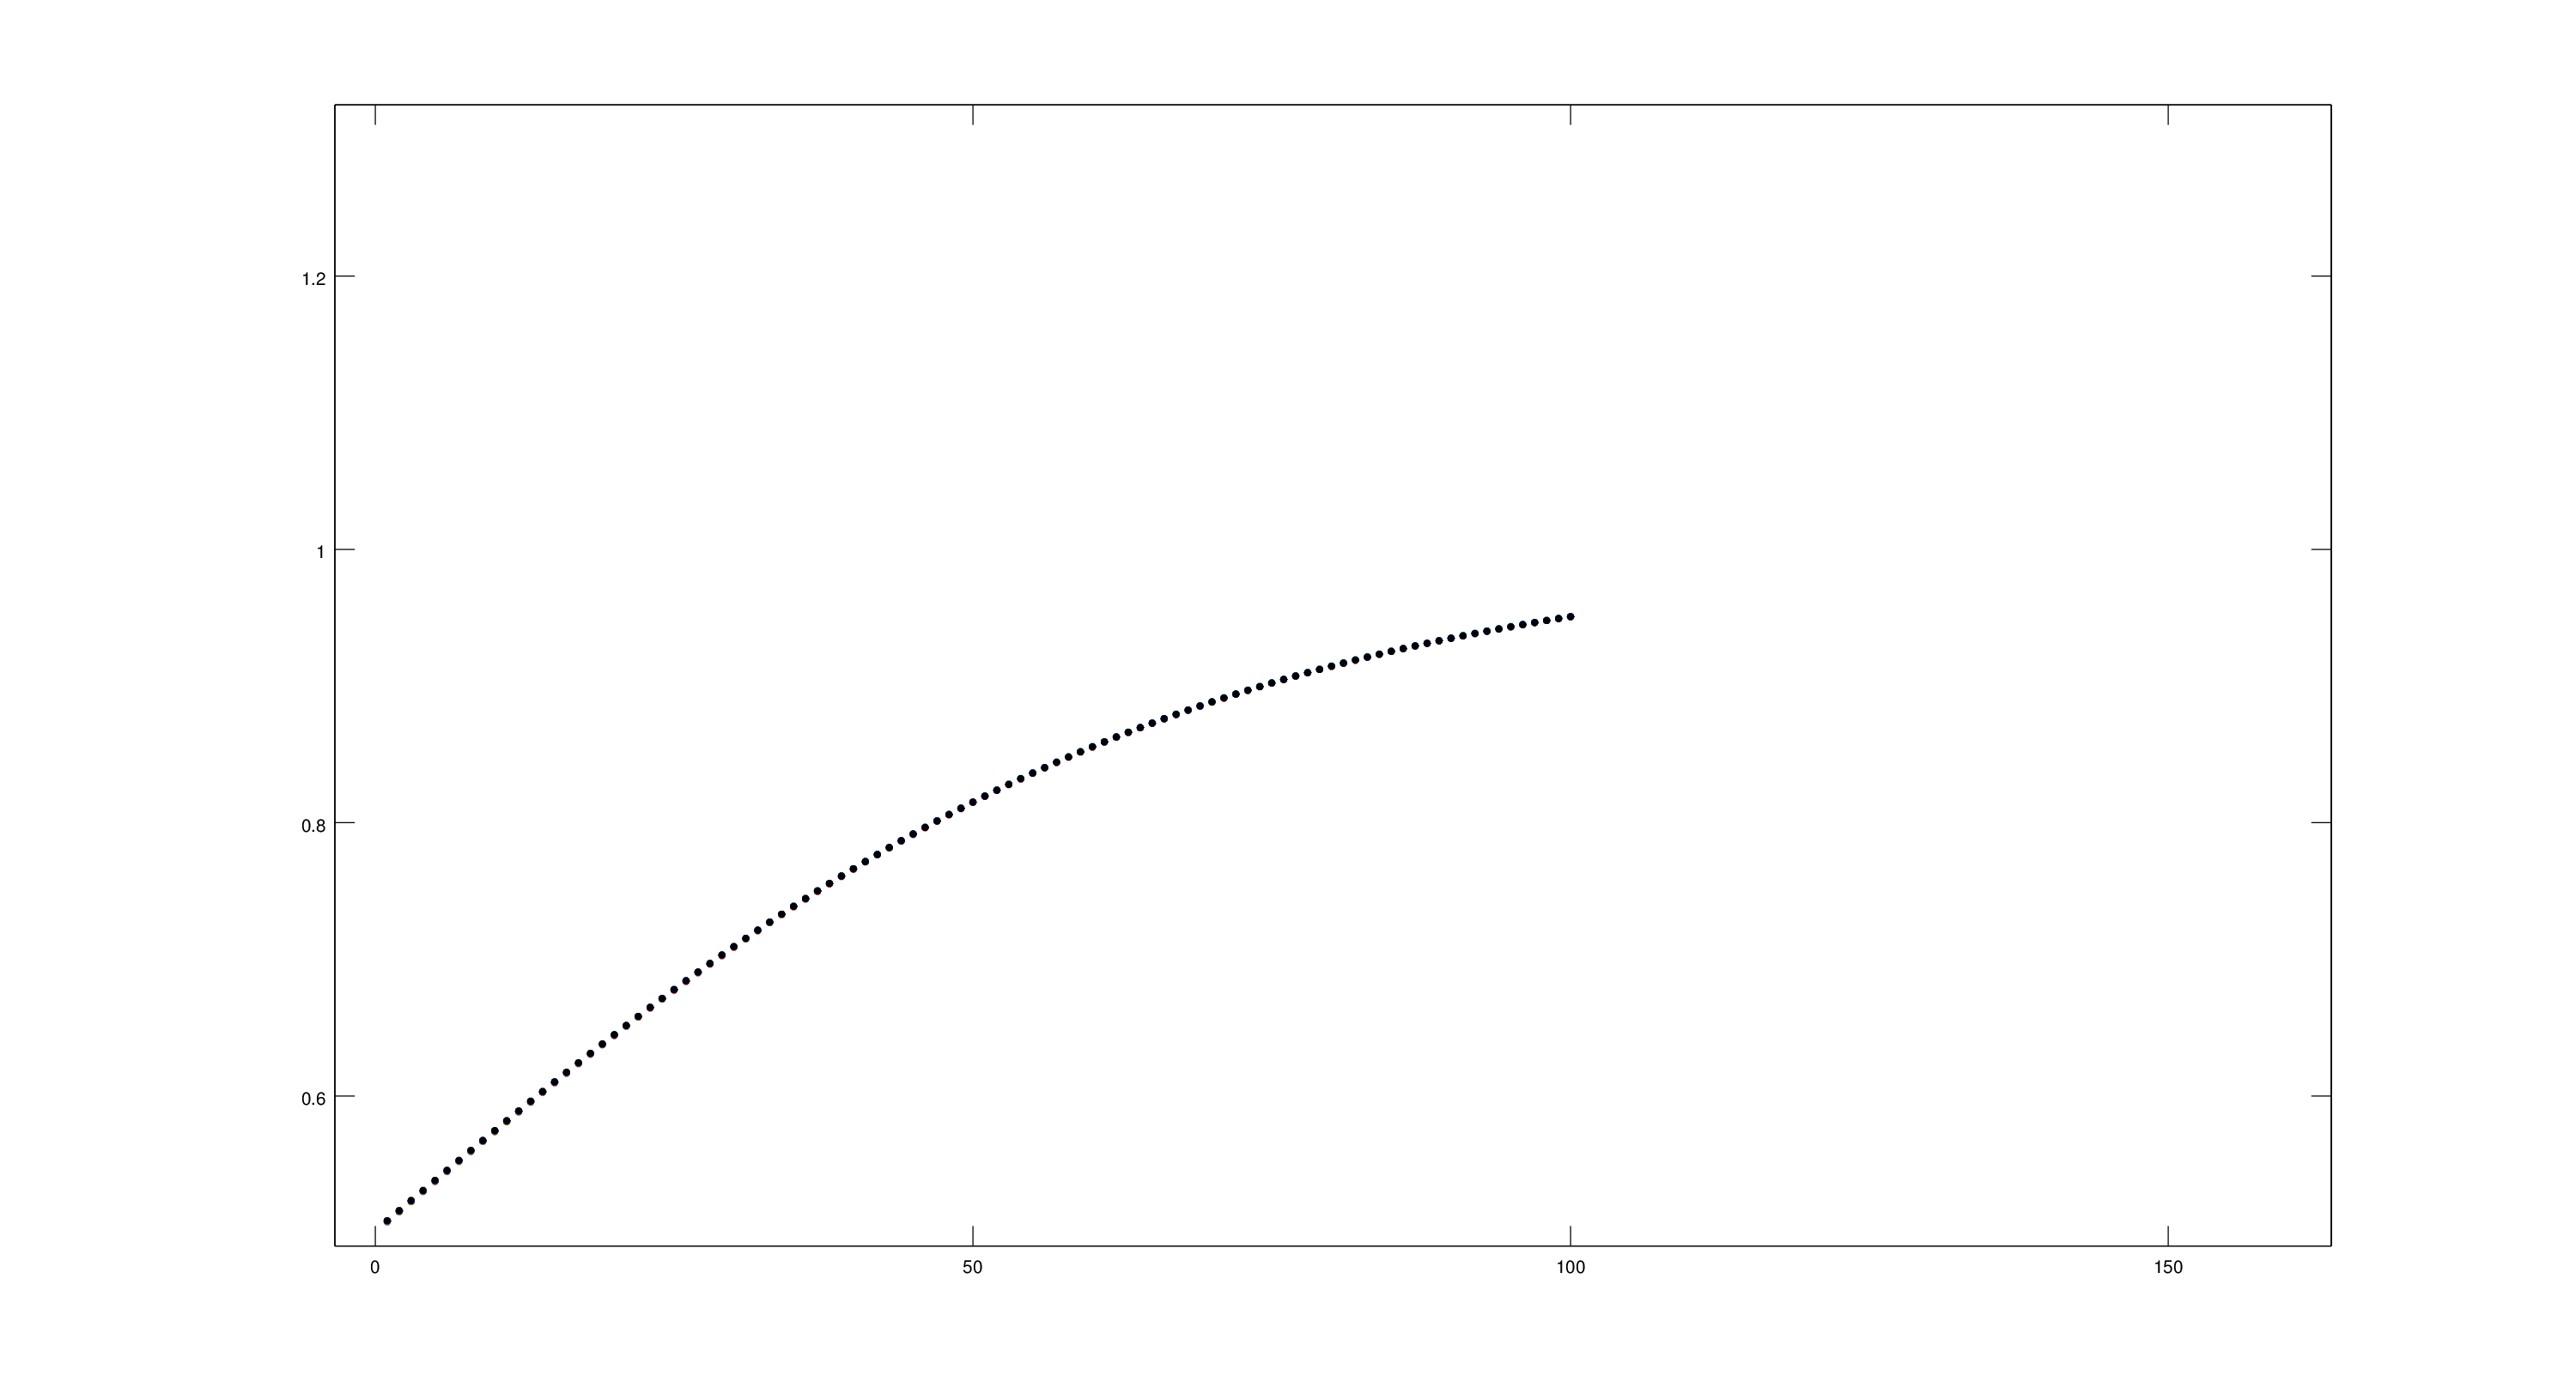
\includegraphics[scale=0.35]{plot1}\\
	Die Kurven überlagern sich sehr stark:\\
	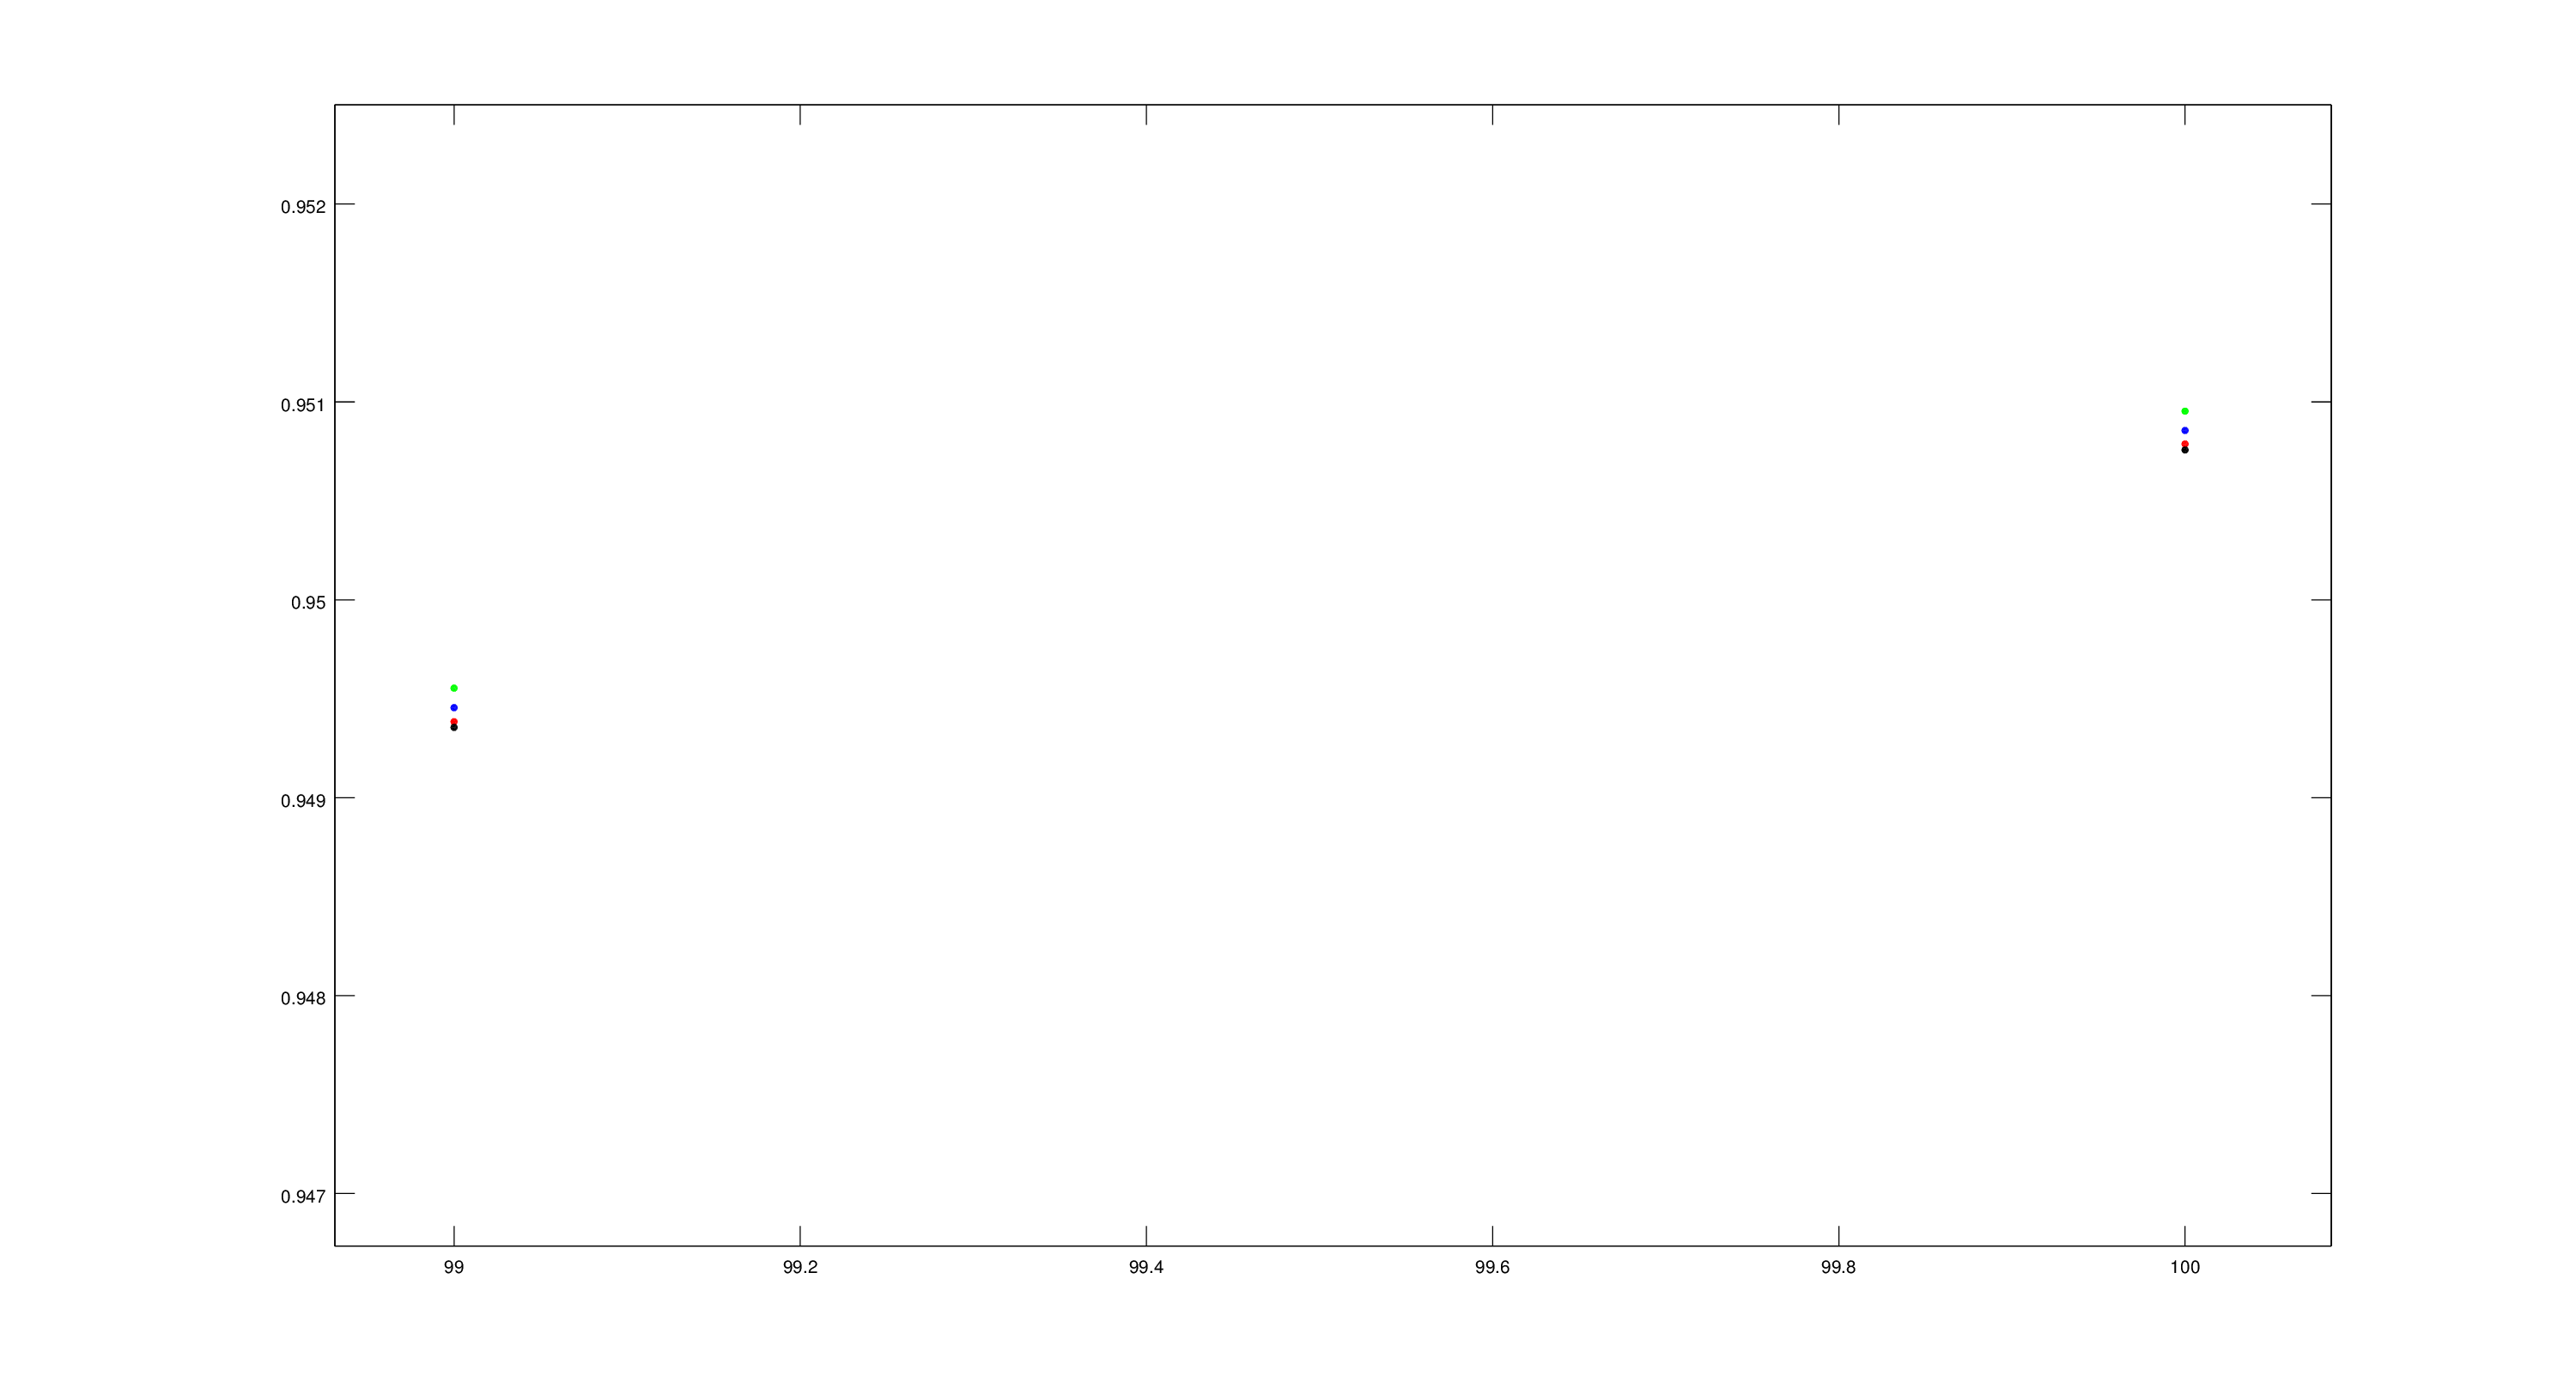
\includegraphics[scale=0.35]{plot2}\\
\end{document}